As explained in Section \ref{sec:sensors}, sensors need to be functionalized with a recognition element which confers selectivity and specificity to the device. 

Two different strategies and recognition elements were used in this project: in a first protocol, an ion-selective membrane was dropcasted on the gate for the detection of ammonium ion, then a different approach was used to functionalize the gold electrode with histamine aptamers with a thiol-modified terminal. 

\subsection{Ion-selective membrane for ammonium detection}
\label{sec:amm_membrane}

\begin{figure}[ht]
    \centering
    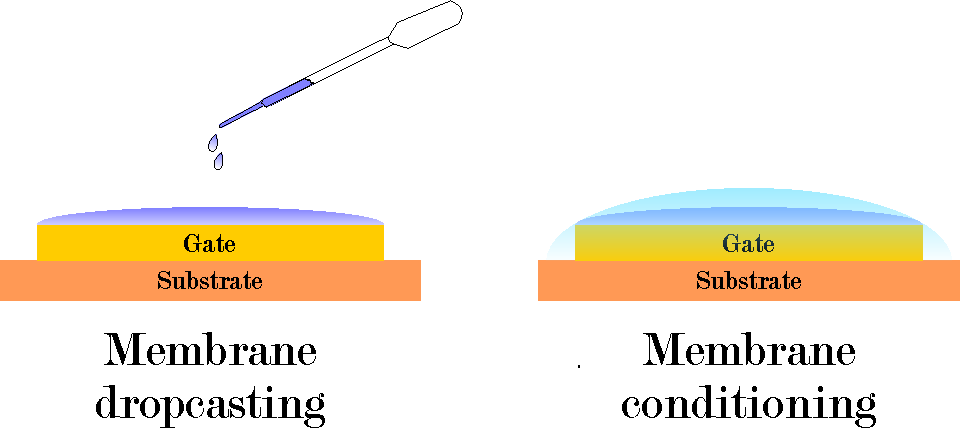
\includegraphics[width=0.6\textwidth]{figures/chapter2/functionalization/Fig11_functionalizationMembrane.pdf}
    \caption{Illustration of the functionalization process with an ion-selective membrane: the membrane was prepared in liquid form, dissolving the reagents in THF, thus it was possible to dropcast it. The optimization of the process led to the deposition of \SI{9}{\micro\l} of solution on the gate, which was then let dry in a refrigerator overnight. Once the THF was fully evaporated, the membrane was conditioned \SI{24}{\hour} in \SI{1}{mM} \amm{}, diluted in 1X PBS. This step primed the ionophore and led to a more sensitive device.}
    \label{fig:functionalizationMembrane}
\end{figure}

Selective detection of ammonium was reached through the use of an ionophore-containing membrane. The composition of this membrane is substantially different than that of the stabilizing membrane, albeit being equally PVC-based. This membrane was composed of \SI{0.2}{\%} nonactin, the ammonium ionophore (\SI{0.23}{\mg}), \SI{30.8}{\%} PVC (\SI{35.42}{\mg}), \SI{69}{\%} ortho-nitrophenyl octyl ether (O-NPOE) (\SI{79.35}{\mg}, \ie{} \SI{76.3}{\ul}) as plasticizer. In the same way as before, these reagents were dissolved in \SI{1}{\ml} THF and processed \SI{5}{\min} in ultrasound sonicator, \SI{5}{\min} of vortexing, and an additional sonication step of \SI{30}{\min} for complete mixing. The membrane solution was then stored at \SI{4}{\celsius} up to one week in a parafilm-sealed vial to prevent THF evaporation; the shelf life is much shorter in this case due to the presence of the nonactin, which loses functionality in a short span of time. 
In the same way as for the stabilizing membrane, the solution needed to be sonicated \SI{1}{\min} before using it, in order to ensure homogeneity, and then rapidly placed in ice; also in this case it was necessary to slow down solvent evaporation for a better control over the dropcasting process.
For the functionalization, \SI{9}{\ul} of the membrane solution were dropcasted onto the gate, then left to dry overnight in a refrigerated environment. 
Once the membrane was set, a first morphological characterization was carried out through visual inspection, optical microscopy and profilometry (see Figure \ref{fig:gateMembraneCharacterization}). Through this assessment, it was possible to assert that the membrane dries translucent, 
Before the electrical characterization, the membrane underwent a \SI{24}{\hour} conditioning step in a \SI{1}{mM} ammonium solution prepared in 1X PBS; although the chemicophysical processes are not fully explained, it is believed that this works as priming of the ionophore, thus making the devices more sensitive a the measurements more reliable. In case the measurements were not taken immediately after conditioning, the membrane had to be reconditioned in the same medium, this time only \SI{2}{hour} before use.

\begin{figure}[hb]
    \centering
    \subfloat[Optical microscopy image of the gate membrane\label{fig:gateMembrane}]{
        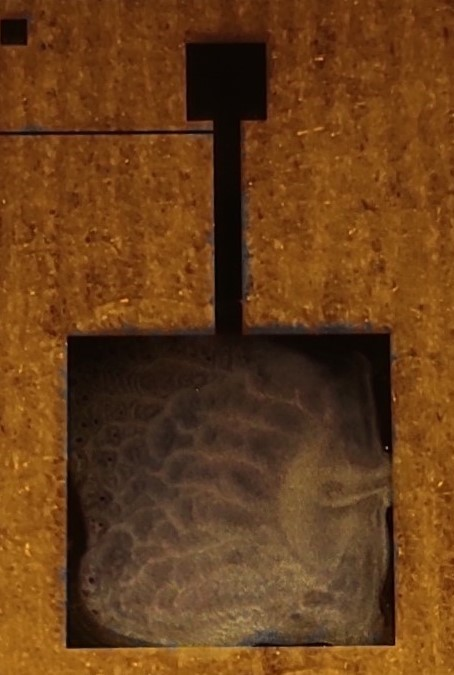
\includegraphics[height=4cm]{figures/chapter2/functionalization/gateMembrane.jpg}
    } \quad
    \subfloat[Profilometry of the gate membrane\label{fig:gateProfil}]{
        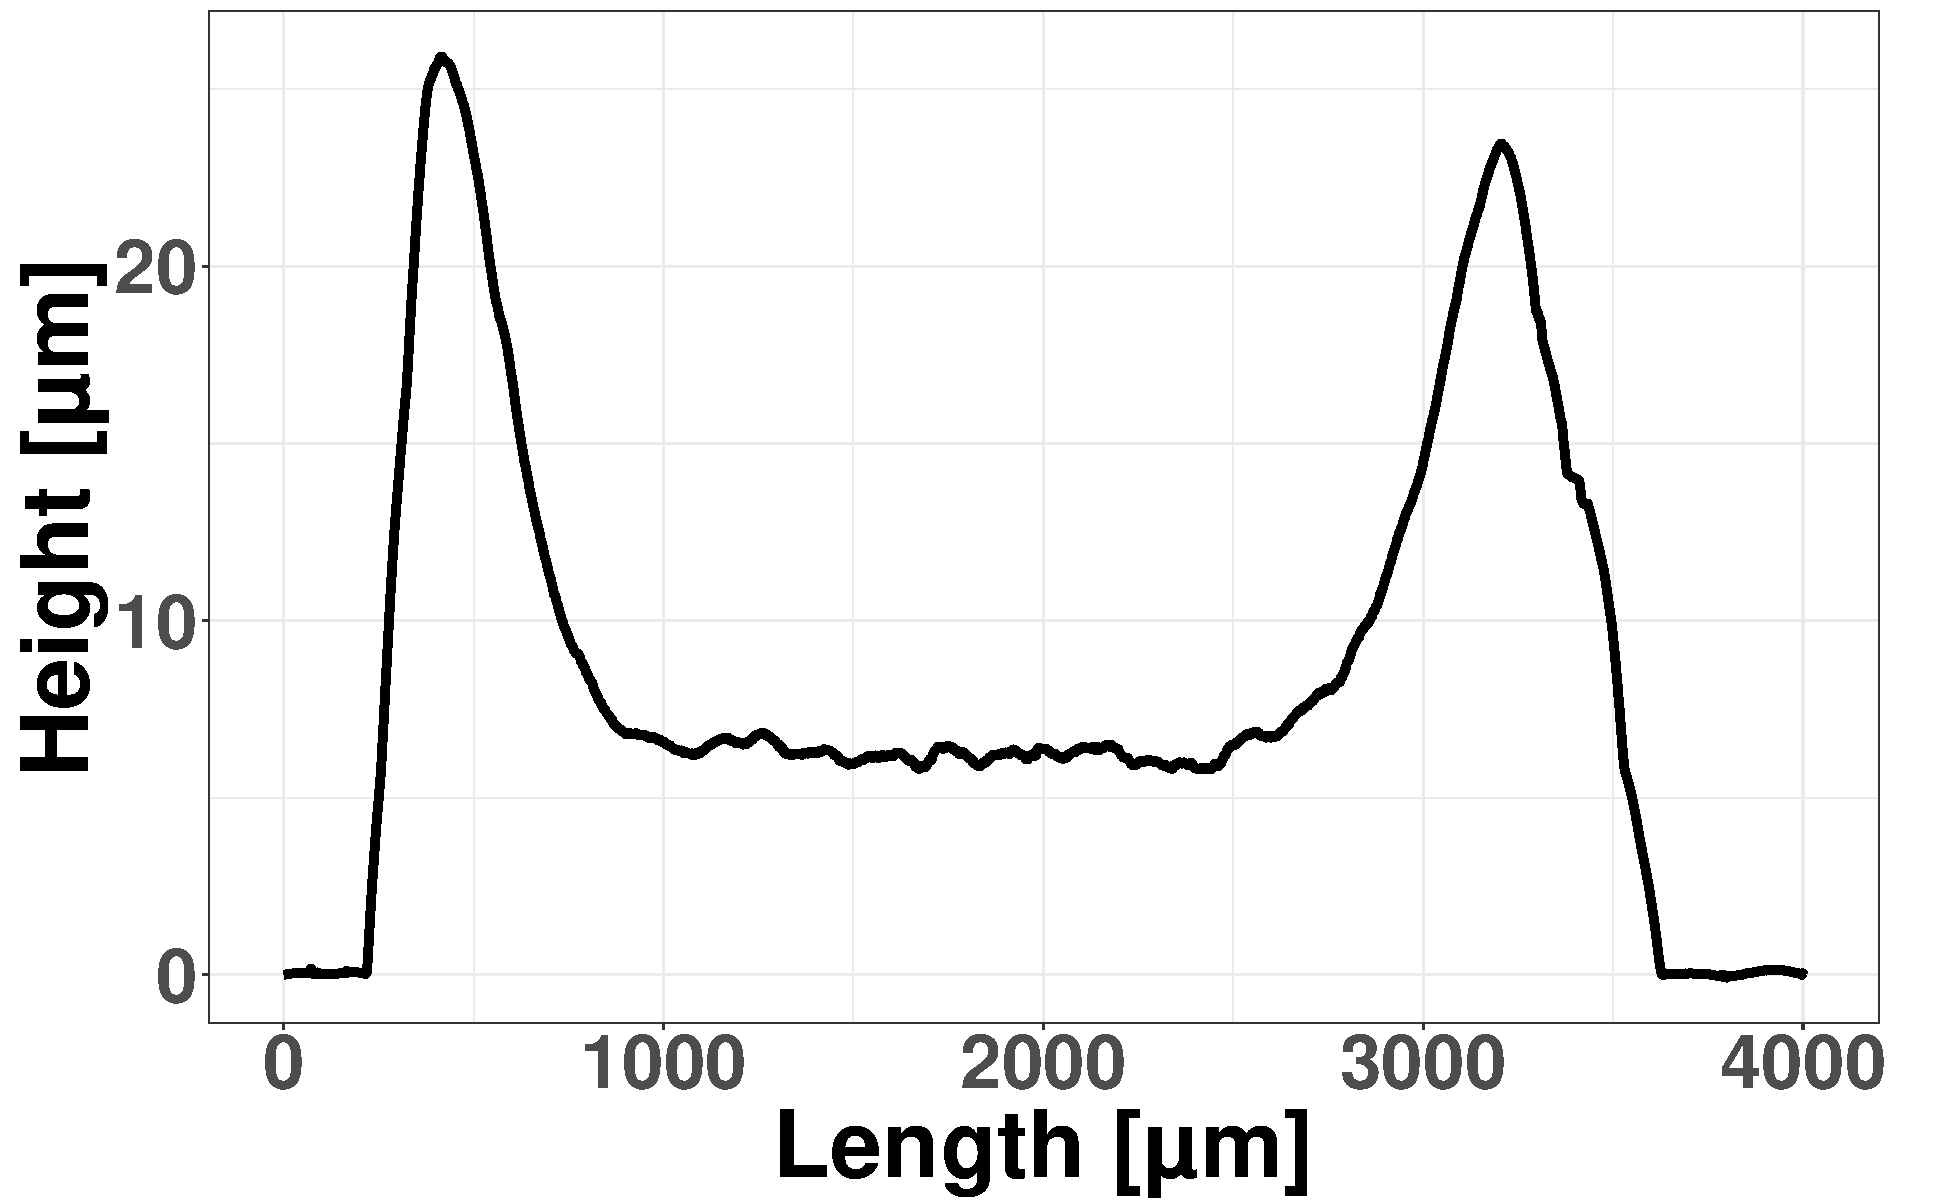
\includegraphics[width=0.4\textwidth]{figures/chapter2/functionalization/gateProfil.pdf}
    }
    \caption{Morphological characterization of the ammonium-sensing membrane. (a) Optical microscopy image showing the membrane as dropcasted on the gate: the membrane covers the entire surface and appears translucent when dry. (b) Profilometry analysis: the membrane has an average thickness of \SI{10.0 \pm 6.0}{\um} and the coffee ring effect is very evident.}
    \label{fig:gateMembraneCharacterization}
\end{figure}

\subsection{Aptamers for histamine detection}
\label{sec:hist_aptamers}

\begin{figure}
    \centering
    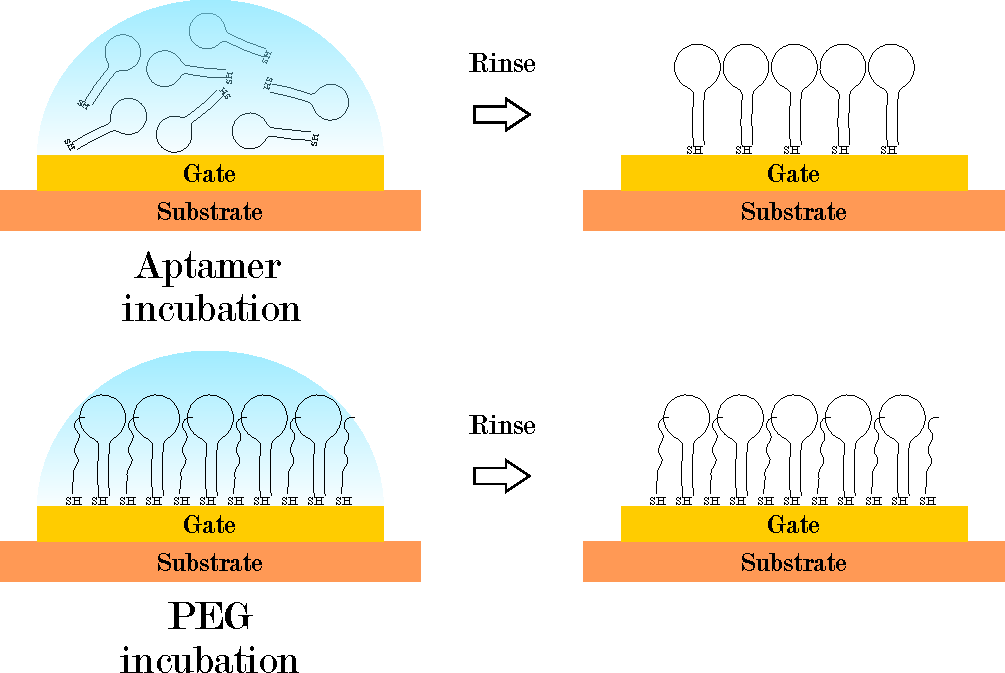
\includegraphics[width=0.6\textwidth]{figures/chapter2/functionalization/Fig12_functionalizationAptamer.pdf}
    \caption{Illustration of the functionalization process with histamine aptamers: the gate is incubated \SI{2}{\hour} in a solution of 1X PBS containing \SI{5}{\micro M} aptamers. The gate is then rinsed 3 times with 1X PBS. A second incubation step occurs, leaving the gate under \SI{1}{mM} PEG} for \SI{2}{\hour}.
    \label{fig:functionalizationAptamers}
\end{figure}

A different protocol had to be developed to functionalize the gate with histamine aptamers. It started by processing the aptamers to prepare the stock solution to be later used:a first centrifugation at \SI{1400}{rpm} for \SI{2}{\min} was needed to collect all the material on the bottom of the vial, then 
\SI{246}{\ul} of 1X PBS were added to achieve a final concentration of \SI{100}{\micro M}. The solution was centrifuged again at \SI{1400}{rpm} for \SI{1}{\min} to collect all the droplets that remained on the walls of the vial, then it was aliquoted in \SI{10}{\ul} and finally it was stored frozen to preserve the DNA. Additional steps in aptamer preparation were required prior to functionalization: indeed, the thiol terminals of the DNA filaments are prone to oxidation, thus forming disulfide bridges (\ce{2RSH <=> RS-SR + 2H+ + 2e-}). The disulfide bonds were reduced by treating the aliquotes with tris(2-carboxyethyl)phosphine (TCEP) at a \SI{50}{X} molar excess (\SI{5}{mM}), incubating them at room temperature for \SI{1}{\hour}. At the end of the incubation period, the solution was diluted to the final concentration of \SI{5}{\micro M}. Prior to gold functionalization, the TCEP was removed using filtrating spin columns: first, the columns were rinsed with water to remove any residues of preserving solution, by centrifuging them three times at \SI{3400}{rpm} for \SI{2}{\min}; then the aptamer-containing solution was centrifuged with the same parameters for the desalting. The resulting solution was then heated to \SI{95}{\celsius} for \SI{5}{\min} to denature DNA, then cooled to room temperature to allow for renaturation and proper folding.

Before aptamer immobilization, the gate needed to be cleaned in order to remove any impurities that could prevent the formation of the thiol-gold bond. The methods tested to this aim included acetone-isopropanol-water rinsing, a modified mild piranha solution (different combinations of \ce{H2O2} - from \SI{50}{\%} down to \SI{6.25}{\%} - and \ce{KOH} - from \SI{50}{mM} down to \SI{12.5}{mM}), and ozone treatment (ranging from \SI{5}{\min} to \SI{15}{\min}). However, none of the tested strategies delivered the desired results: solvent cleaning proved insufficient in removing impurities, piranha solution excessively damaged the surface that needed to be functionalized, and ozone treatment caused extensive damage to the CNT network, negatively impacting their stability and their conductivity. The winning strategy, exploiting ozone cleaning, will be discussed in Section \ref{sec:histamine}.

The gate could be finally functionalized by incubating with the aptamer solution for \SI{2}{\hour}, followed by an additional \SI{2}{\hour} incubation with polyethylene glycol (PEG), a blocking agent that prevents aspecific interactions on the gate. After each incubation, the gate was throughly rinsed with 1X PBS to ensure that only the covalently attached material remained on the gold surface. Before measurement, the functionalized devices were left stored with 1X PBS to prevent drying and denaturation of aptamers and PEG. To follow the functionalization process, cyclic voltammetry (CV) and electrochemical impedance spectroscopy (EIS) were employed, as discussed in the following section.

